\chapter[Embasamento Teórico]{Embasamento Teórico}

\section{Engenharia de Requisitos} 

Por se tratar de uma área que se encontra entre o abstrato e o concreto, Westfall \cite{westfall_5w2h}, em seu estudo, busca definir os diferentes porquês da existência da Engenharia de Requisitos, sendo:

\begin{itemize}
    \item O que é?: são os requerimentos responsáveis pela definição do que o \textit{software} deve fazer (\textit{requisito funcional}\footnote{Declarações de serviços que o sistema deve prover, como deve reagir para entradas e como deve se comportar em situações especificas \cite{Sommerville10}.}) e possuir (\textit{requisitos não funcionais}\footnote{Restrições aos serviços ou funções oferecidas pelo sistema. Aplicam-se ao sistema como um todo \cite{Sommerville10}.}) para agregar valor para os seus \textit{stakeholders}\footnote{Grupo de pessoas interessadas no produto, podendo ser cliente, usuários etc.}; Existem vários níveis e tipos diferentes de requisitos, que são mostrados na Figura \ref{lev_tipo_req}:
    
    \begin{figure}[htb]
        \begin{center}
            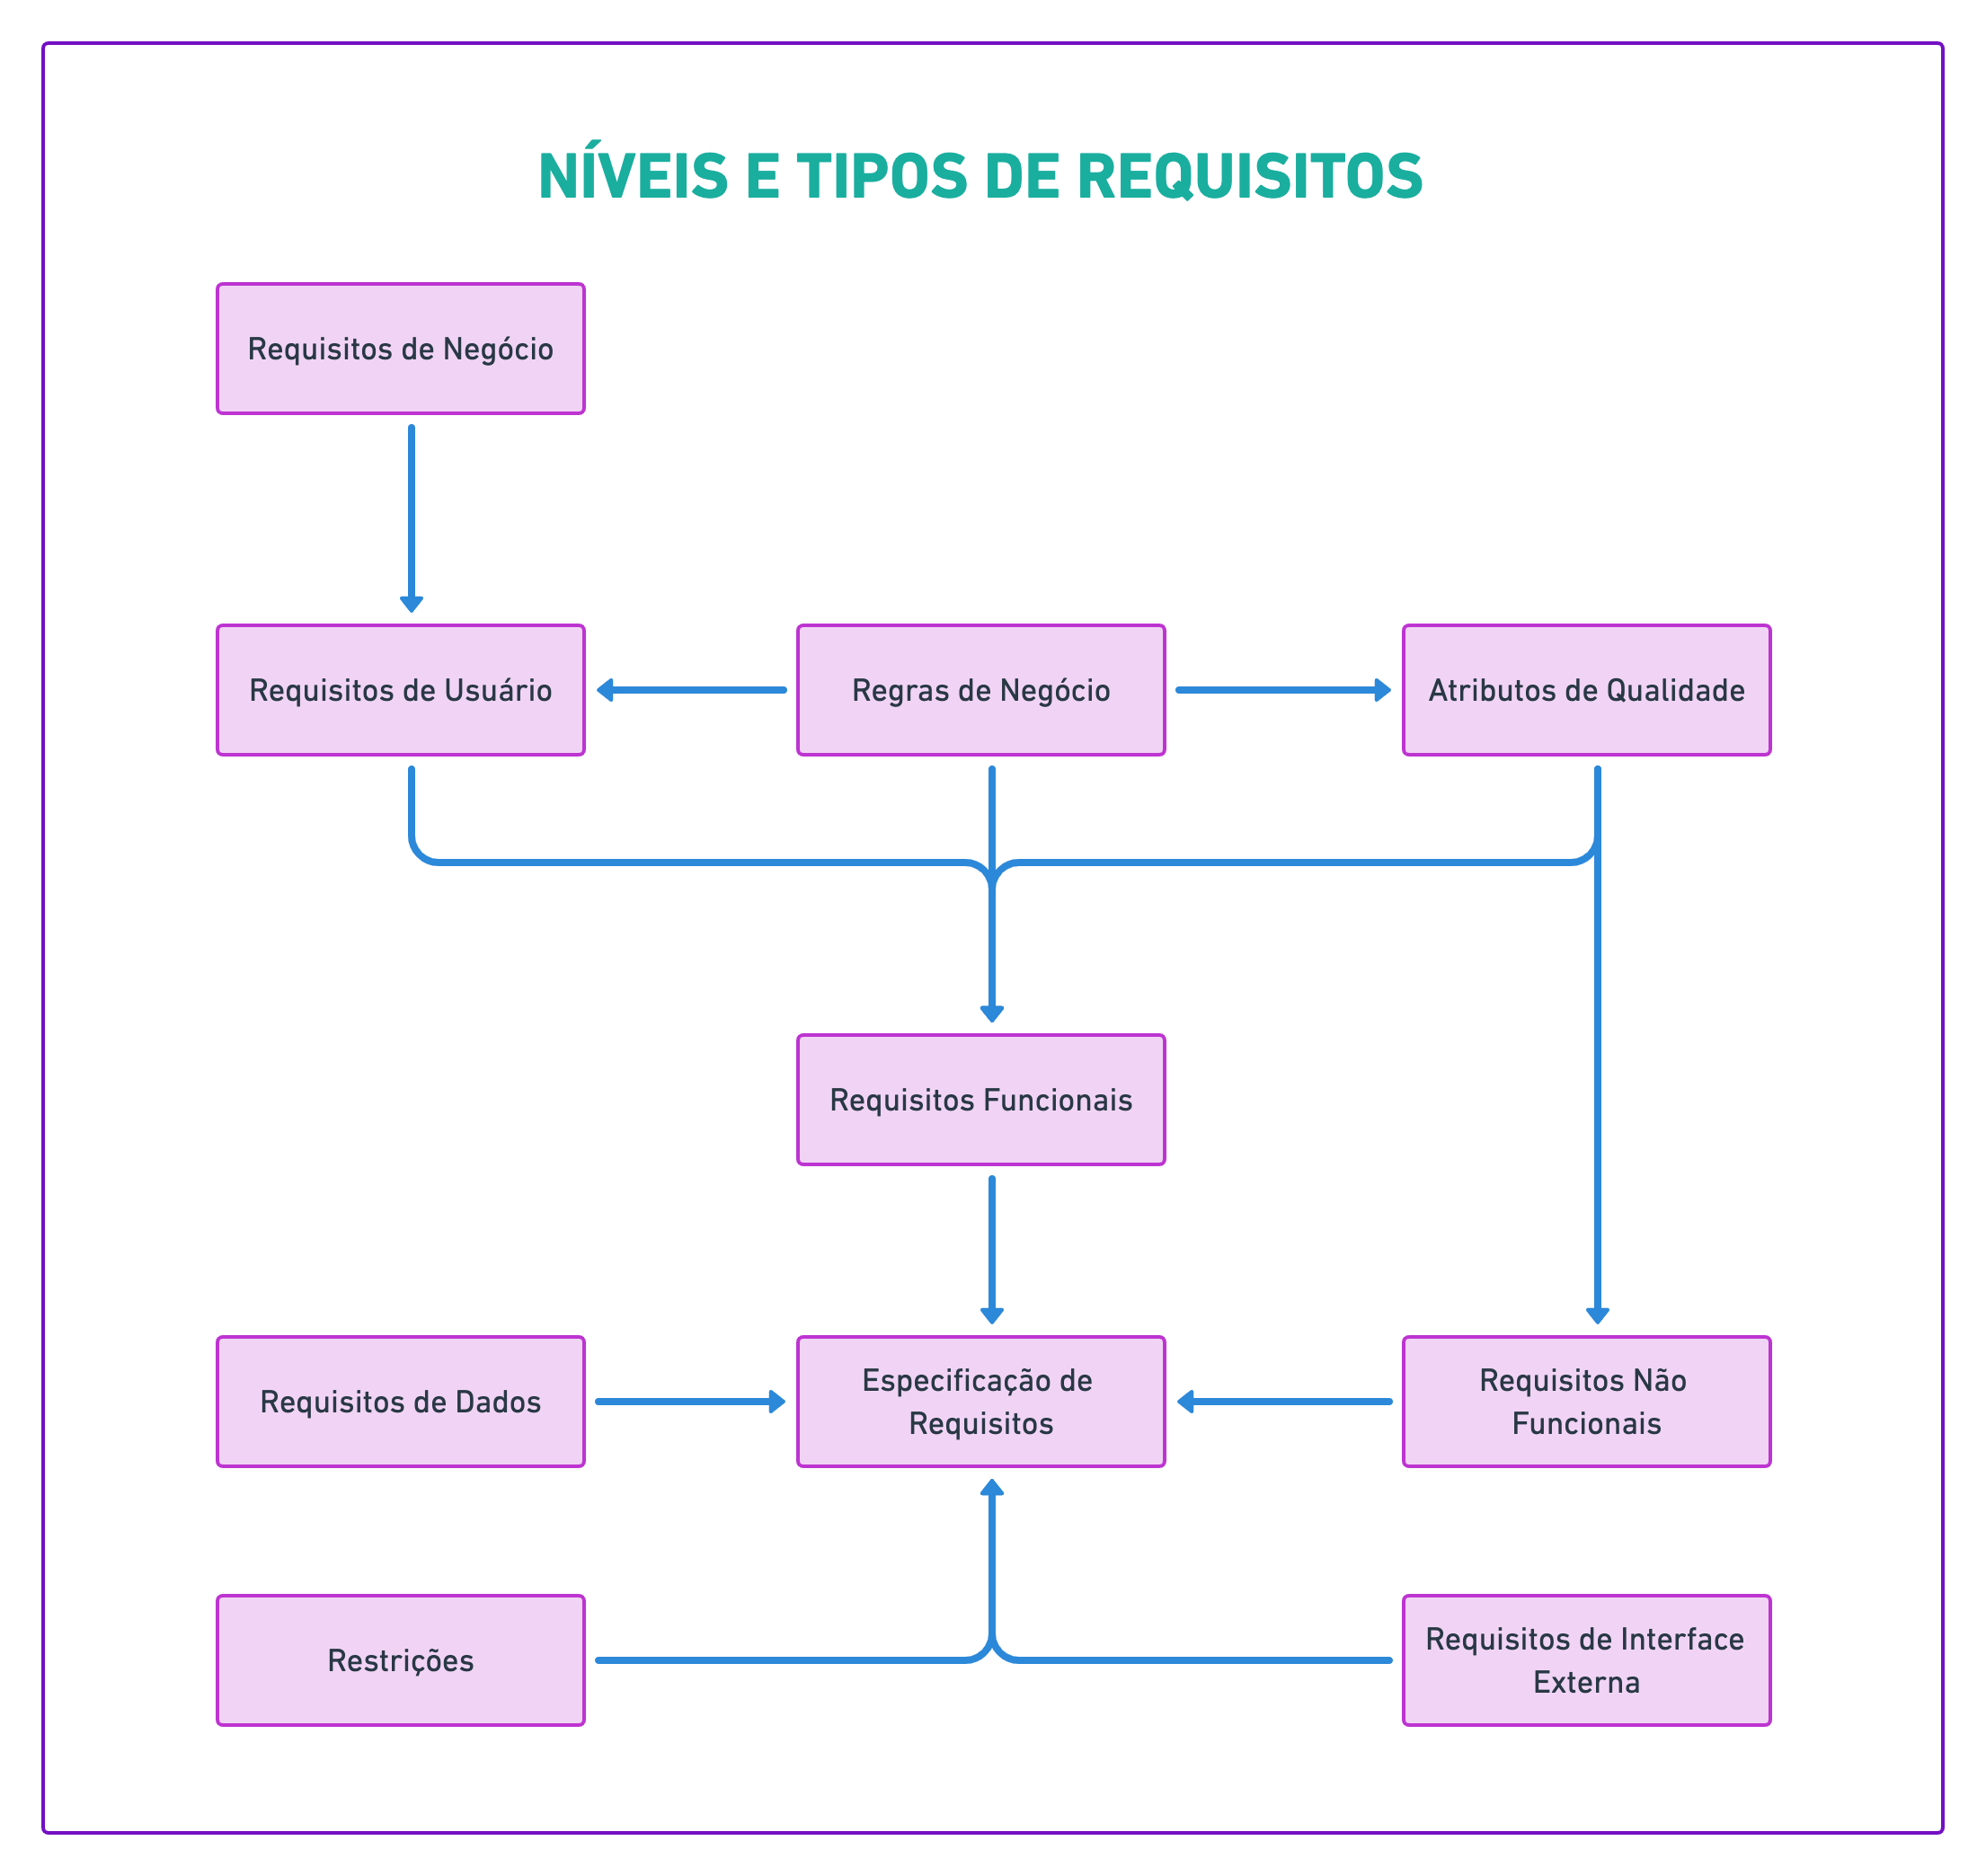
\includegraphics[width=12cm, height=10cm, keepaspectratio]{figuras/lev_tipo_req.png}
            \caption{{Níveis e Tipos de Requisitos. Fonte: \cite{westfall_5w2h}}}
            \label{lev_tipo_req}
        \end{center}
    \end{figure}
    
    \begin{itemize}
    
        \item Os \textbf{requisitos de negócio} definem, de forma direta, quais são os problemas que devem ser resolvidos e por que o produto de \textit{software} está sendo desenvolvido;
        
        \item Os \textbf{requisitos de usuário} têm o objetivo de visualizar as funcionalidades do produto de \textit{software} a partir da perspectiva do usuário. De forma resumida, eles definem o que o \textit{software} deve realizar para que os usuários atinjam seus objetivos;
        
        \item Os \textbf{requisitos funcionais} de produto definem as funcionalidades do \textit{software} que devem ser implementadas para que os usuários consigam realizar suas tarefas de forma fácil;
        
        \item As regras de negócio são declarações sobre a forma da empresa fazer negócio, ou seja, elas refletem as políticas, os padrões, as práticas, os regulamentos e as diretrizes de negócio;
        
        \item Os \textbf{atributos de qualidade} no nível de usuário definem requisitos não funcionais que determinam o produto de \textit{software}. Incluem confiabilidade, disponibilidade, segurança, manutenibilidade, portabilidade, usabilidade, dentre outros;
        
        \item Os requisitos\textbf{ de interface externa}, de forma objetiva, definem o fluxo de informações através de interfaces compartilhadas;
        
        \item As \textbf{restrições} têm o objetivo de mostrar quais destas limitações foram colocadas pelo fornecedor ao projetar e desenvolver o \textit{software};
        
        \item Os requisitos de dados definem os itens de dados específicos que devem ser introduzidos como parte do produto de \textit{software}.
    
    \end{itemize}
    
    \item Para que serve? : um dos grandes nomes da engenharia de \texit{software}, Fred Brooks, afirma que
        \begin{citacao}
            A parte mais difícil da construção de um sistema de \textit{software} é decidir precisamente o que deve ser feito. Nenhuma outra parte do trabalho conceitual é tão  custoso quanto estabelecer detalhadamente os requisitos técnicos, incluindo todas as interfaces para os usuários, para os computadores, e para os outros sistemas do \textit{software}. Nenhuma outra parte do trabalho prejudica tanto o sistema se for feita de maneira errada. Nenhuma outra parte é tão difícil de ser retificada posteriormente \cite[p.~199]{brooks1995mythical}.
        \end{citacao}
    Assim, pode-se entender o quão crítico é esse fase do processo de desenvolvimento de \texit{software}, contexto que se insere esse trabalho;
    
    \item Para quem?: os \textit{stakeholders} são indivíduos que impactam ou que são impactados pelo produto de \textit{software} e, portanto, possuem um nível de influência sobre o produto. Dentro desse contexto, existem diferentes perspectivas relacionadas à atuação de cada indivíduo, sendo os mais comuns:
    
    \begin{itemize}
        \item Os Analistas de Requisitos são essenciais dentro dessa área pelo fato deles serem responsáveis pela elicitação, análise e especificação dos requisitos, além de comunicar os requisitos aos desenvolvedores e às partes interessadas;
    
        \item Os Arquitetos de \textit{Software} são essenciais por criarem toda a arquitetura do \textit{software} a partir dos requisitos elicitados e por dizerem como vai ser implementado;
    
        \item Já os desenvolvedores são responsáveis pela implementação o produto de \textit{software}, traduzindo os requisitos em funcionalidades concretas;
    
        \item Os Testadores de \textit{Software} têm o objetivo de usar os requisitos elicitados como base, e criar casos de teste para que o produto de \textit{software} seja testado sob condições específicas, afim de detectar defeitos para que, após os testes, passem confiabilidade de que o produto de \textit{software} esteja funcionando de acordo com as características estabelecidas;
    
        \item Os Gerentes de Projeto são responsáveis pelo planejamento e pelo monitoramento de todos os envolvidos no projeto, além de guiar o time de desenvolvimento de \textit{software} para que o produto final seja entregue com todos os requisitos definidos anteriormente e,
    
        \item O Gerente do Produto é uma peça fundamental dentro desse processo, pois revisa todas as mudanças propostas; analisa os riscos e os impactos que podem vir a ocorrer, e aprova ou desaprova quaisquer mudanças, garantindo que essas mudanças foram implementadas e validadas.
    \end{itemize}
    
    \item Quando?: a maior parte do processo da Engenharia de Requisitos é feita nas primeiras fases do ciclo de vida do produto, contudo não deve ser restrito somente a esse período, uma vez que novos requisitos vão surgindo e o projeto deve se adaptar às novas realidades, pois deve ser um processo iterativo. Esse aspecto está ligado ao gerenciamento de requisitos, o qual necessita avaliar como novas requisições influenciam no desenvolvimento do projeto, assim como elencar os riscos e impactos causados por essas alterações. Posteriormente, após a aprovação, ocorre a implementação da nova funcionalidade. Durante a fase de desenvolvimento, estes requisitos devem ser usados como critérios para testar o produto e validar a correta implementação das funcionalidades. Os requisitos de negócio devem ser os primeiros a serem modelados, seguidos dos requerimentos de usuário e, por fim, os de produto, e
    
    \item Como?: A Engenharia de Requisitos de \textit{software} é um processo bem definido, com etapas claras e repletas de documentações que possam registrar e orientar o desenvolvimento do produto. O desenvolvimento e a gerência dos requisitos são dois grandes processos dentro deste escopo. A Figura \ref{eng_req_flux} representa bem essas etapas e subetapas do processo da Engenharia de Requisitos que vão ser mais bem especificadas no decorrer deste trabalho.
    
    \begin{figure}[htb]
        \begin{center}
            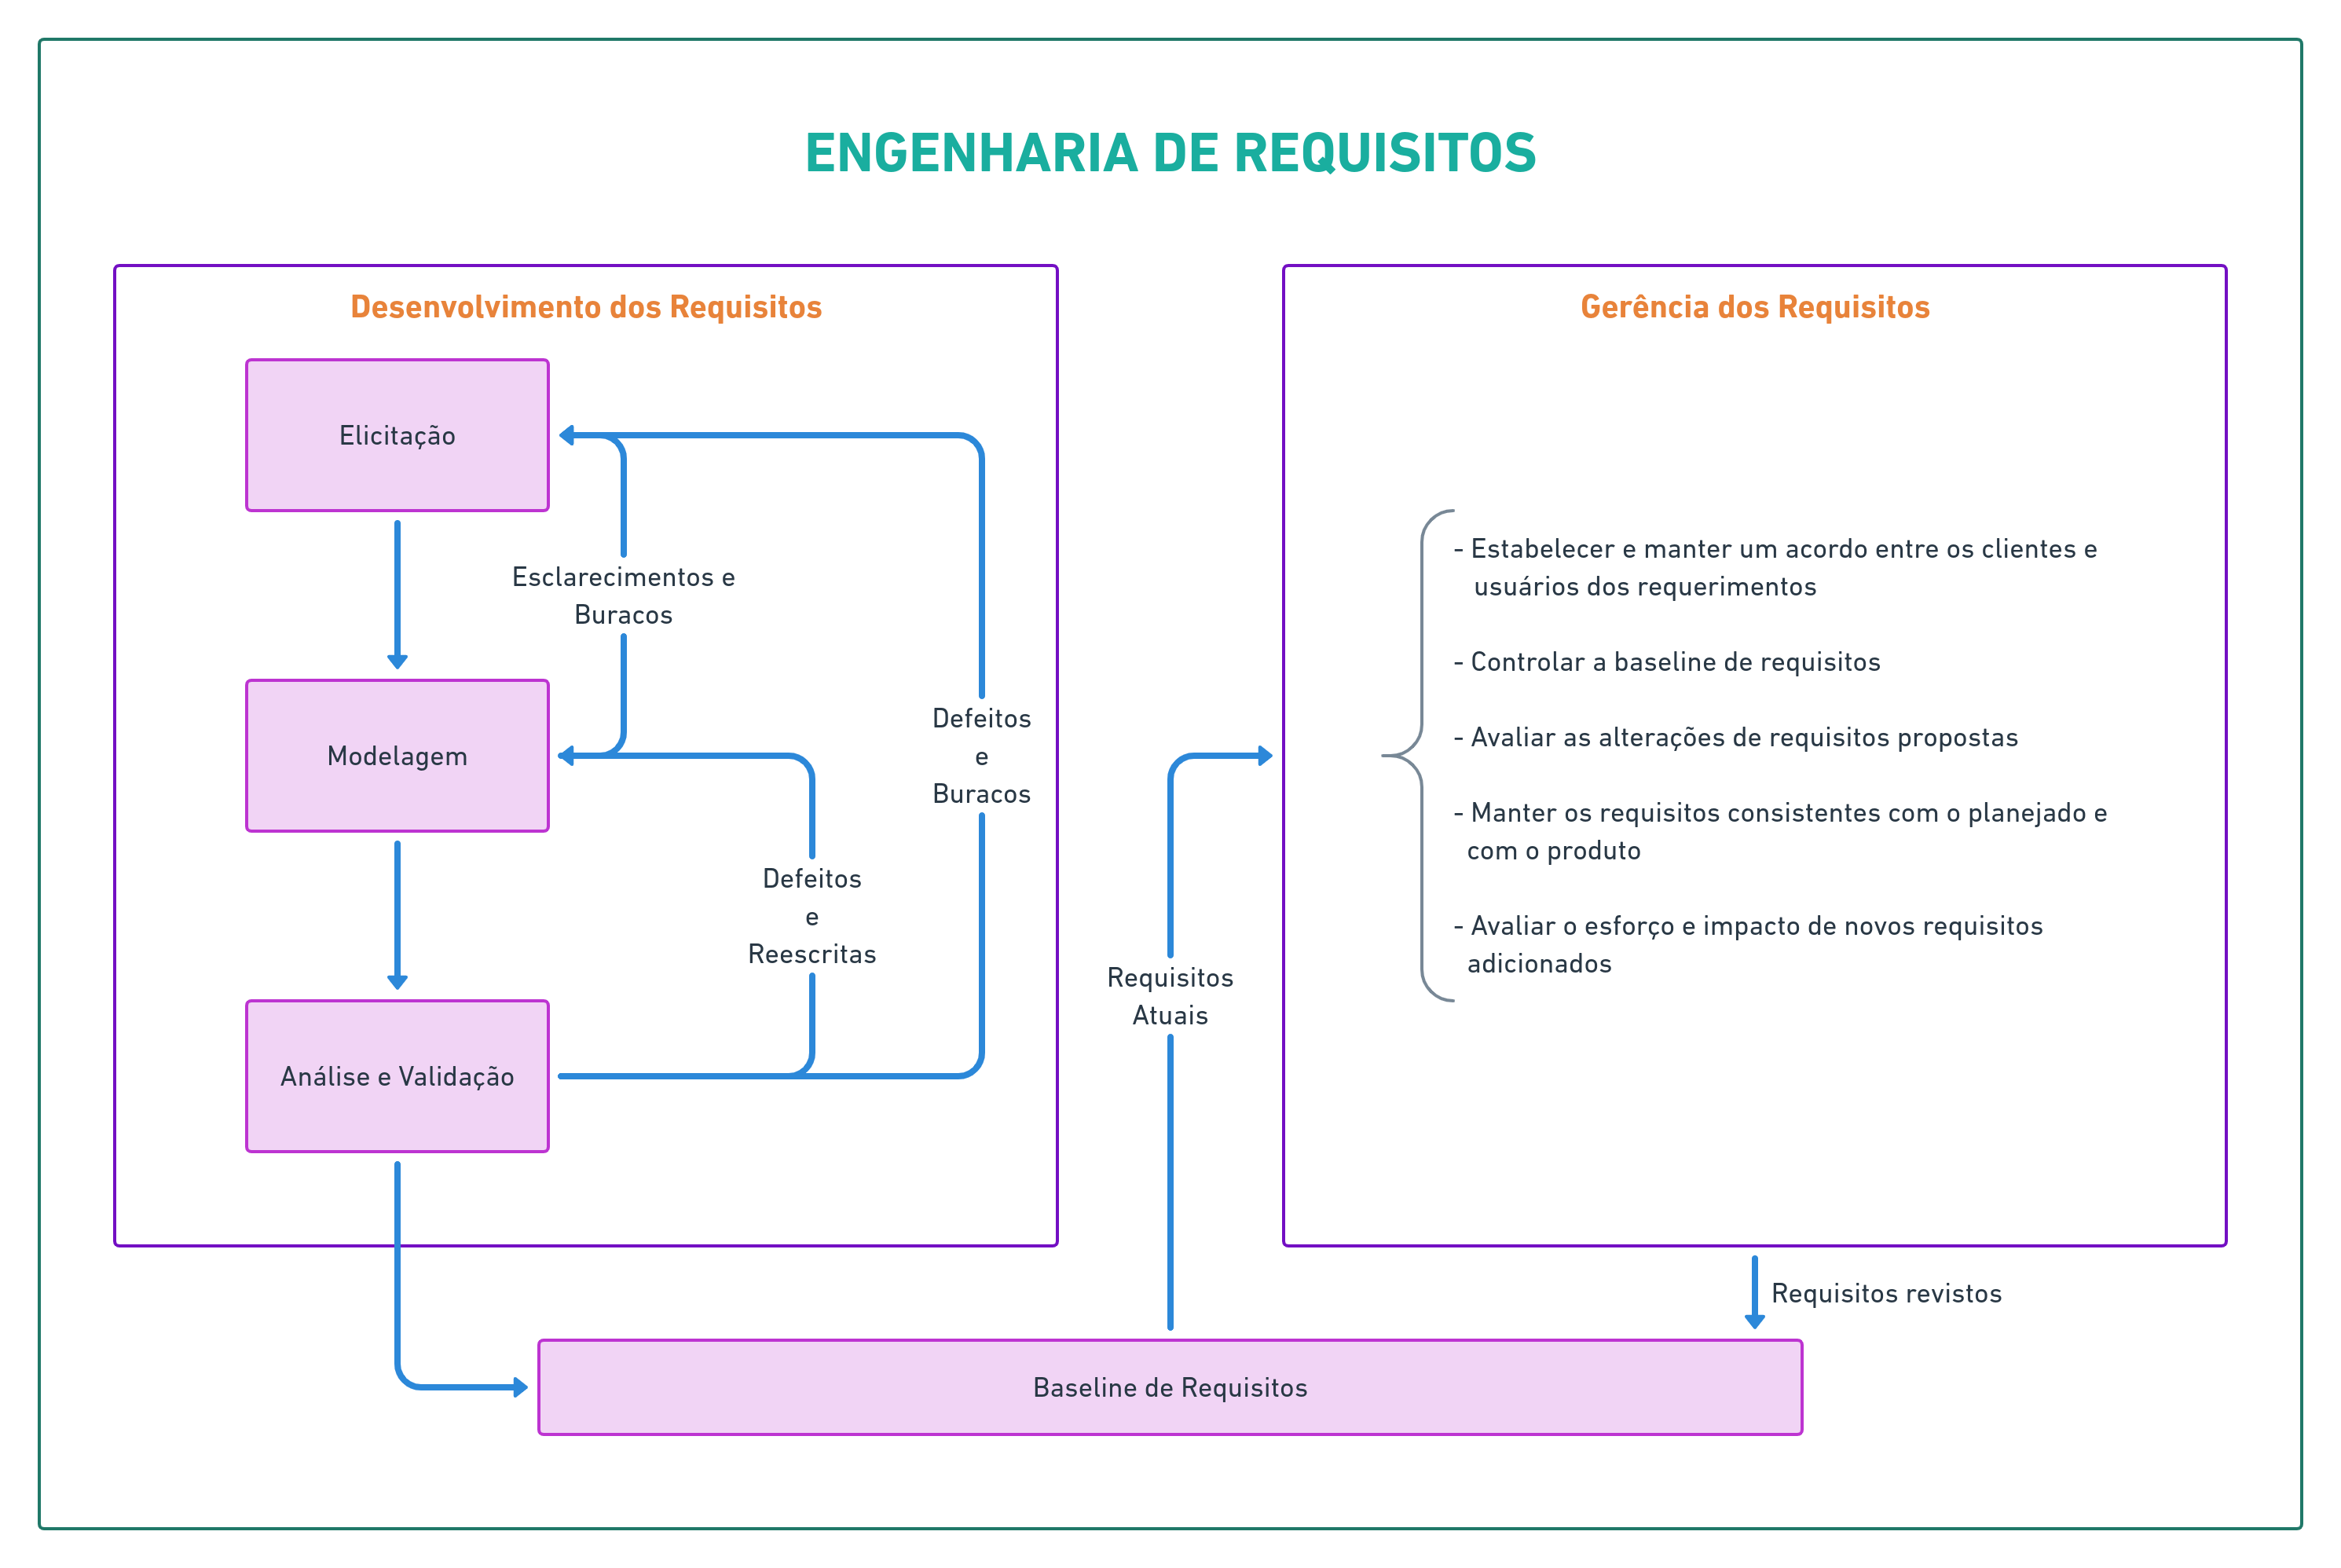
\includegraphics[width=12cm,height=12cm,keepaspectratio]{figuras/Introducao/eng_req_fluxo.png}
            \caption{{Fluxo da Engenharia de Requisitos. Fonte: adaptado de \cite{westfall_5w2h}}}
            \label{eng_req_flux}
        \end{center}
    \end{figure}
    
\end{itemize}

Como vimos, a Engenharia de Requisitos é uma área essencial dentro da construção de um produto de \textit{software}. Existem vários processos e várias técnicas utilizadas para que o produto final seja desenvolvido com qualidade, evitando problemas no futuro.

Algum dos processos e técnicas utilizadas dentro da Engenharia de Requisitos serão citadas a seguir.

\section{Pré-rastreabilidade}

A Pré-rastreabilidade se preocupa, de forma objetiva, em rastrear um requisito até a sua origem. De forma exemplificada, quando um requisito é alterado, usa-se a pré-rastreabilidade para investigar as informações que foram utilizadas para obtê-lo, ou seja, para saber qual a pessoa interessada, quais técnicas ou quais documentos o requisito foi extraído, etc \cite{pinheiro2004requirements}.

\subsection{Rich Picture}
A \textit{Rich Picture} é uma ilustração que se assemelha a um desenho animado, com o objetivo de identificar as partes interessadas, suas preocupações e uma parte da estrutura subjacente. É uma ferramenta para registrar e raciocinar sobre os aspectos do contexto de trabalho e como eles afetam o produto  \cite{10.1145/274430.274434}. Além disso, ela se baseia em rascunhar desenhos e usar textos curtos e objetivos para expressar um momento, um desejo, uma atividade, dentre outras necessidades.

\subsection{5W2H}
O 5W2H é uma ferramenta empregada no planejamento estratégico de empresas, análise de negócios, elaboração de planos de negócios, planejamento estratégico e outras áreas de gestão. Tem o objetivo de descrever um plano de ação com as atividades que precisam ser desenvolvidas com o máximo de clareza possível. Essa ferramenta baseia-se na elaboração de uma tabela formada por 7 perguntas: O quê? Por que? Quem? Onde? Quando? Como? Quanto custa? \cite{rabuskeuso}.


\begin{itemize}
    \item O quê?: Que ação será executada;
    \item Por que?: Por que a ação será executada;
    \item Quem?: Quem irá participar da ação;
    \item Onde?: Onde será executada a ação;
    \item Quando?: Quando a ação será executada;
    \item Como?: Como a ação será executada;
    \item Quanto custa?: Quanto custa para executar a ação.
\end{itemize}

\section {Elicitação}

\label{sec:elicitacao}

A Elicitação de Requisitos é o processo relacionado com as atividades que permitem a compreensão de metas, objetivos e motivos para a construção de um novo sistema de \textit{software} e a identificação de todos os requisitos das partes interessadas que facilitarão o sistema a ser desenvolvido \cite{elliott2012software}. Além disso, as informações coletadas durante a elicitação de requisitos geralmente precisam ser interpretadas, analisadas, modeladas e validadas antes do início da implementação do sistema \cite{nuseibeh2000requirements}.

\subsection{Brainstorming}
O \textit{Brainstorming} ou "Tempestade de Ideias", por ser uma técnica de grupo, tem o objetivo de coletar o maior número de ideias acerca de um determinado tema ou questão. É utilizada, geralmente, na fase de planejamento de um projeto. Propõe que um grupo de pessoas se reúnam a fim de colaborar para uma "tempestade de ideias", onde cada ideia é somada para que se forme um longo processo de sugestões e discussões. Vale ressaltar que nenhuma ideia, inicialmente, é criticada ou julgada \cite{mazzotti2012exploraccao}. O \textit{Brainstorming} é usada para gerar novas ideias, deixando a mente livre para aceitar todas as ideias que foram sugeridas e, assim, permitir a liberdade para a criatividade \cite{batista2003taxonomia}.

\subsection{Questionário}
O Questionário é uma técnica de coleta de informações que permite aos envolvidos no projeto estudar atitudes, crenças, comportamentos e características do público alvo que podem ser afetados pelo sistema atual e pelo sistema proposto \cite{kendall1992systems}. É uma técnica que deve ser realizada com muita cautela. A elaboração das perguntas que vão constituir o questionário é um processo engenhoso, complexo e delicado. Um questionário mal elaborado pode, facilmente, levar a conclusões erradas que acabam sendo prejudiciais para o projeto que está sendo desenvolvido \cite{bastosjunior}.

\subsection{Protótipo de Baixa Fidelidade}
Um Protótipo, segundo \cite{Sommerville10} "é uma versão inicial de um sistema de \textit{software}, usado para demonstrar conceitos, experimentar opções de projeto e descobrir mais sobre o problema e suas possíveis soluções". É muito significativo dentro do processo de Engenharia de Requisitos pelo fato de ajudar na elicitação e validação dos requisitos de \textit{software} e para estudar soluções específicas do \textit{software}.

\subsection{\textit{Storytelling}}

O \textit{Storytelling}, ou simplesmente História, é um artefato que busca por meio da análise da descrição de algum processo ou tarefa realizado em algum contexto para realizar a extração de \textit{features} do sistema. Vale ressaltar que, nesse contexto, não existe um formato ou estrutura pré-definida, mas possuem descrições de altos níveis de uso do sistema. São muito usadas em contexto de dar o panorama geral do sistema  \cite{Sommerville10}.

Vale ressaltar que nosso cérebro, segundo estudos, são mais propensos ao aprendizado proveniente de histórias. Por retratar a experiência de quem conta, validado por suas próprias experiências, as narrativas proporcionam um retrato realista e lógica de algo vivido por seu interlocutor. Isso proporciona um entendimento com uma carga de sentimentos e fatos que podem ser usados para a extração de requisitos mais ricos  \cite{storytelling}.

\subsection{Entrevista}
A Entrevista é uma das técnicas mais utilizadas por possuir uma comunicação mais natural entre as pessoas. As Entrevistas são usadas para a obtenção de conhecimento sobre um determinado tema/domínio através de perguntas feitas aos usuários especialistas, além de trazer muitas informações aos desenvolvedores do projeto \cite{batista2003taxonomia}. De acordo com \cite{Sommerville10}, elas podem ser de dois tipos:
\begin{itemize}
    \item Fechadas: seguem um conjunto de perguntas pré-definidas;
    \item Abertas: não se tem uma agenda pré-definida.
\end{itemize}
Na prática, geralmente, as entrevistas são um mesclado dos dois tipos.

\subsection{Análise de Protocolo}
A Análise de Protocolo consiste em pedir a uma pessoa para ela se envolva em uma tarefa e fale em voz alta o seu processo de pensamento para que ocorra uma extração de possíveis requisitos do sistema \cite{goguen1993techniques}. Usuários alegam que esse tipo de linguagem pode ser considerada uma "verbalização direta do processo cognitivo específico". Vale ressaltar que a Análise de Protocolo está sujeita a problemas de interpretações pelos analistas \cite{belgamo2000estudo}.

\section {Modelagem}

\label{sec:modelagem}

Esta parte do processo da Engenharia de Requisitos consiste em estruturar os requisitos que foram levantado no período da elicitação(\ref{sec:elicitacao}) de forma sistemática. De acordo com \cite{Sommerville10}, os requisitos "devem ser claros, inequívocos, fáceis de entender, completos e consistentes".

Vale ressaltar que os documentos gerados nesta fase devem ser de fácil entendimento para os \textit{stakeholders} do projeto, sem que hajam detalhes técnicos de implementação ou arquitetura do sistema \cite{Sommerville10}.

\subsection{Backlog}

\label{sec:backlog}

O \textit{Backlog} do Produto é um artefato essencial dentro da Engenharia de Requisitos, na metodologia ágil e no ciclo de desenvolvimento de um produto, pois todos os requisitos constam nele. Em uma definição mais concreta, o \textit{Backlog} é uma lista ordenada e emergente de tudo que é necessário no produto, ou seja, é a única fonte dos requisitos \cite{carolipaulo2021}. Todas as funcionalidades são descritas no \textit{Backlog} e é o que o cliente espera receber no fim do projeto.

\subsection{NFR}
O NFR Framework (\textit{Non-Functional Requirements}) é um artefato que visa tratar os requisitos não funcionais expressando-os sistematicamente e usando-os para guiar o processo de desenvolvimento do \textit{software}. Este consiste em dar uma abordagem orientada a procedimentos para requisitos não funcionais, onde estes podem ser retratados como metas a serem atingidas \cite{coutoproposta}. Além disso, de acordo com \cite{chung2012non}, o "NFR \textit{Framework} usa os requisitos não funcionais como segurança, precisão, desempenho e custo para conduzir o processo geral de design. O Framework visa colocar os requisitos não funcionais em primeiro lugar na mente do desenvolvedor".

\subsection{House of Quality}

O \textit{House of Quality} ou Casa da Qualidade é um processo de planejamento sistemático elaborado para compreender de forma explícita a "voz do cliente" no \textit{design} do produto. Esta pode ser vista como uma ferramenta gráfica para compreender e avaliar a relação entre as preocupações do cliente e as do desenvolvedor \cite{Howard_1}.

\begin{figure}[H]
    \begin{center}
        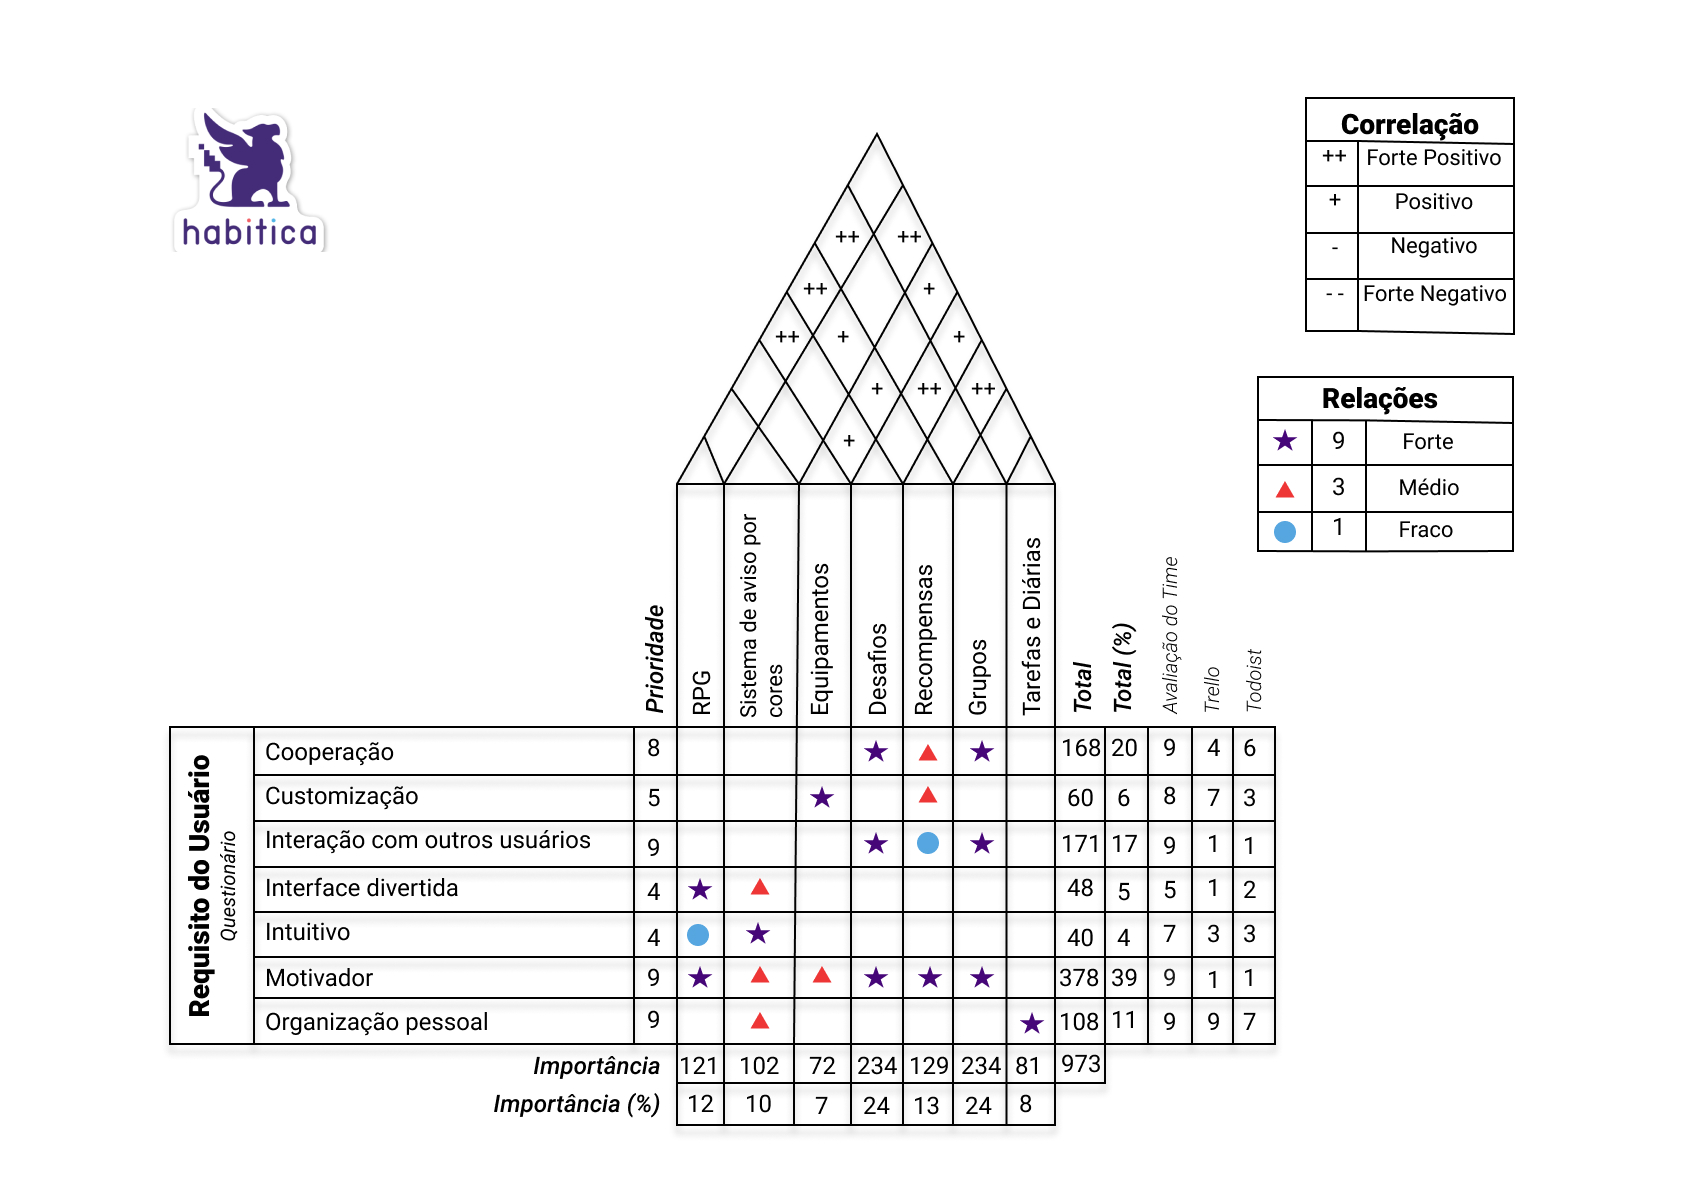
\includegraphics[scale=0.55]{figuras/referencial_teorico/HOQ.jpg}
        \caption{{HOQ exemplificado do App Habitica. Fonte: Autores}}
        \label{grafo_1}
    \end{center}
\end{figure}

É composto por 5 partes, sendo elas:

\begin{itemize}
    \item No centro são comparados os requisitos técnicos propostos com as necessidades do cliente classificando sua relação;
    \item À direita se encontra uma comparação dos concorrentes com relação ao produto da empresa, sobre as necessidades do cliente, nela é possível comparar os diferentes parâmetros dos concorrentes com o produto e ter uma noção da qualidade do produto;
    \item À esquerda se encontram as necessidades dos clientes levantadas com um peso de prioridade, para ser possível atender a maioria dessas necessidades;
    \item Em baixo são comparados todos os requisitos dos produtos concorrentes com o da empresa da mesma forma que as necessidades, e
    \item Em cima se encontram as correlações de todos os requisitos técnicos, sendo ali onde é determinado os parâmetros conflitantes, neles que a equipe deve ponderar e descobrir o meio termo no desenvolvimento.
\end{itemize}

\subsection{Léxicos}
O Léxico é definido como um conjunto dos vocábulos de uma língua, dispostos em ordem alfabética e com as respectivas significações. Uma notação na modelagem de requisitos que usa a descrição de termos via léxico é o LAL (Léxico Ampliado da Linguagem). Trata-se de uma técnica que consiste em definir os símbolos de uma linguagem. Esses símbolos são descritos em \textbf{noções}\footnote{Significa o símbolo, é colocado no sentido denotativo da linguagem.} e \textbf{estados}\footnote{Efeito/uso/ocorrência do símbolo na aplicação, que pode ser colocado no sentido conotativo da linguagem.} \cite{leite1993strategy}. Cada Léxico pode ser definido em somente um tipo, que são eles:

\begin{itemize}
    \item Objetos: são aqueles que se relacionam com outros objetos;
    \item Verbos: são as ações;
    \item Estados: são gerados a partir de ações (verbos).
\end{itemize}

\section {Verificação}

Se trata de uma etapa rigorosa do processo da Engenharia de Requisitos, no qual os artefatos gerados na modelagem(\ref{sec:modelagem}) são revisados. Essa etapa é essencial, pois dentro do contexto do desenvolvimento de um \textit{software}, uma refatoração é mais custosa que a inspeção de um artefato previamente a implementação. São usadas diversas técnicas nesta etapa que podem ser realizadas de acordo com a necessidade e a estratégia adotada pelo verificador. \cite{verification}.

\section {Pós-rastreabilidade}
A Pós-rastreabilidade consiste em rastrear um requisito para a implementação de um projeto. De forma exemplificada, quando um requisito é alterado, usa-se a pós-rastreabilidade para investigar o impacto desta mudança. Por fim, tem-se o conhecimento de onde o requisito está implementando e qual foi o caminho percorrido por ele. Nesse sentido, o \textit{Backward-from} é utilizado e consiste em ligar os principais requisitos do sistema com as suas origens, por exemplo, com uma pessoa, uma instituição, etc \cite{pinheiro2004requirements}.

\section{Priorização (MVP)}
O MVP (\textit{Minimum Viable Product}) é definido como a versão mais simples de um produto que pode ser colocado para negociação. Determina quais são as funcionalidades mais importantes e que agregam mais valor ao produto para que ele seja validado e efetivado pelo usuário final \cite{carolipaulo2018}.

\section {Rastreabilidade}
A rastreabilidade é um tópico essencial dentro da Engenharia de Requisitos, pois é utilizado para providenciar relações entre requisitos, arquitetura e implementação final do sistema, além de possibilitar uma compreensão dos relacionamentos de dependência entre os requisitos propostos. Dessa forma, a rastreabilidade pode ser implementada como um conjunto de ligações entre os requisitos \cite{sayao2006rastreabilidade}.

A rastreabilidade tem o objetivo de acompanhar e descrever o ciclo de um requisito de duas formas:
\begin{itemize}
    \item Pré-rastreabilidade: documentar o contexto a partir do qual emergem os requisitos;
    \item Pós-rastreabilidade: vincula os requisitos à arquitetura do sistema e sua implementação.
\end{itemize}

\section{Grafos}

Grafo é uma estrutura de dado que é formado por um conjunto de vértices e arestas. É uma maneira de codificar relações emparelhadas entre um conjunto de objetos. Consiste em uma coleção V de nós e uma coleção E de arestas, onde as arestas juntam dois nós \cite{Kleinberg+Tardos:06a}. A imagem abaixo mostra a representação de um Grafo com os vértices (A, B, C, D e E), suas respectivas arestas e os pesos (3, 5, 9, 2, 1, 1, 6).

\begin{figure}[H]
    \begin{center}
        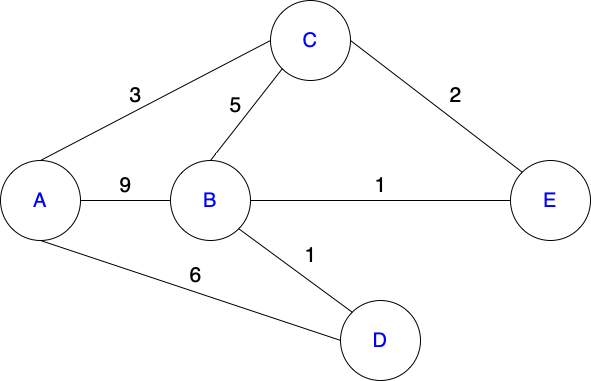
\includegraphics[scale=0.45]{figuras/referencial_teorico/Grafo.drawio.png}
        \caption{{Grafo. Fonte: Autores}}
        \label{grafo_1}
    \end{center}
\end{figure}

\subsection{Algoritmo de Menor Caminho}
O Algoritmo de Menor Caminho consiste em calcular, para cada vértice V, a menor distância de S para V, ou seja, a menor soma possível de pesos de arestas que formem um caminho de S para V, onde S e V são vértices dentro de um grafo G. Os Algoritmos de \textit{Djikstra} e \textit{Floyd-Warshall} são os mais famosos para realizar o cálculo da menor distância entre dois vértices \cite{even2011graph}.
